\documentclass[a4paper, 12pt]{article}
\usepackage[a4paper,left=2.5cm,right=3cm,top=2cm,bottom=2cm]{geometry}
\usepackage[ngerman]{babel}
\usepackage[utf8]{inputenc}
\usepackage[]{csquotes}
\usepackage[style=authoryear-comp,backend=biber]{biblatex}
\usepackage{mathptmx}
\usepackage[T1]{fontenc}
\usepackage{relsize}
\usepackage{graphicx}
\usepackage[]{blindtext}
\graphicspath{ {images/} }

\addbibresource{sources.bib}

\author{Lars Eppinger}
\title{Quantifizierung von Code-Qualität mithilfe statischer Code-Analyse}
\date{1. Juni 2020}

\begin{document}
\begin{titlepage}
    \begin{center}
        \vspace*{1cm}
        
        \Huge
        \textbf{Quantifizierung von Code-Qualität mithilfe statischer Code-Analyse}
        
        \vspace{0.5cm}
        \LARGE
        Sind Tools zur statischen Code-Analyse ein akkurater Weg zur Quantifizierung von Code-Qualität in der objektorientierten Programmierung?
        
        \vspace{1.5cm}
        
        \textbf{Lars Eppinger}

        \Large
        178121\\
        DAI-17
        
        \vfill
        
        Fachbeitrag zur Modulprüfung\\Wissenschaftlich angeleitete Berufspraxis
        
        \vspace{0.8cm}
        
        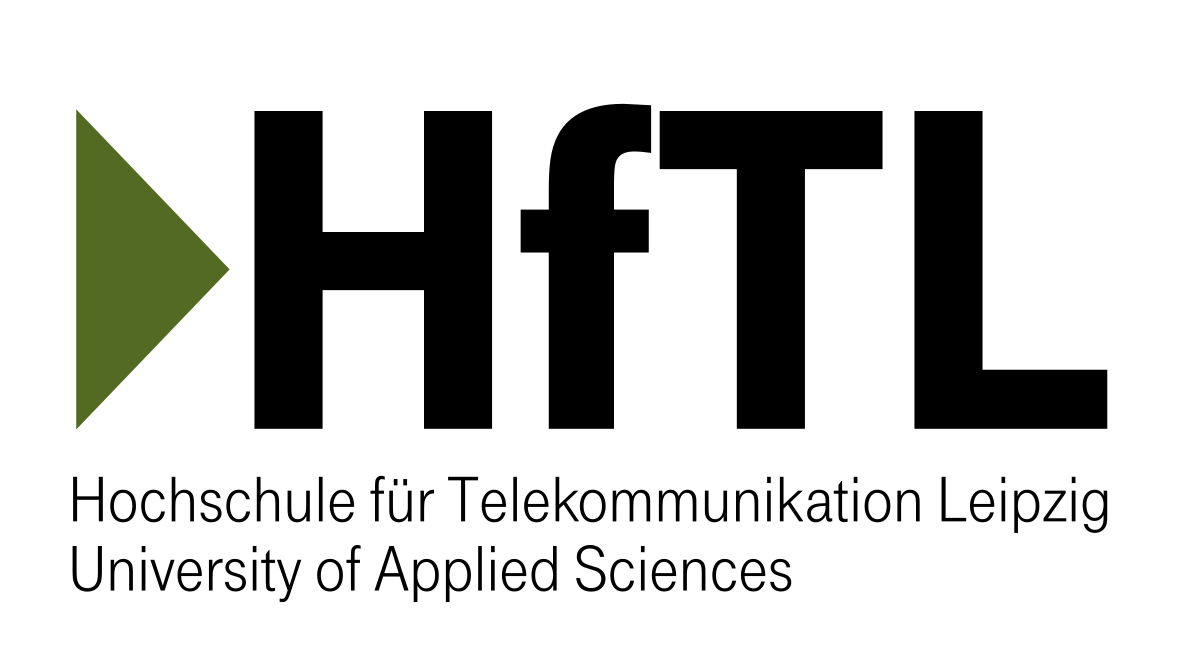
\includegraphics[width=0.4\textwidth{}]{university.png}
        
        \Large
        Hochschule für Telekommunikation Leipzig\\
        1. Juni 2020
        
    \end{center}
\end{titlepage}
\tableofcontents
\newpage

\section{Einführung}
Code-Qualität ist einer der entscheidenden Faktoren über Sicherheit, Wartbarkeit und Maintainability von Softwareprojekten. 
Durch neue Ansätze in der Softwareentwicklung, speziell der agilen Softwareentwicklung, ist es immer wichtiger, hohe Qualität in einer Codebasis sicherzustellen, um die Umsetzung neuer Anforderungen so schnell und fehlerfrei wie möglich zu gestalten.
Immer häufiger kommen für diesen Zweck Tools zur statischen Code-Analyse zum Einsatz.
In dieser Arbeit wird die Frage geklärt, ob das statische Code-Analyse-Tool SonarQube dazu geeignet ist, die Qualität einer Java-basierten Code-Basis zu quantifizieren.

\section{Code-Qualität}
\subsection{Definition}
Als Definitionskriterien für Code-Qualität verwendet diese Arbeit die Attribute für Code-Qualität von \textcite{Linda_softwarequality} und den daraus abgeleiteten Metriken.
Metriken für die Quantifizierung von Code-Qualität müssen nach \textcite{Linda_softwarequality} dazu geeignet sein, die folgenden Attribute eines System zu evaluieren:
\begin{itemize}
    \item Effizienz -- Sind die Konstrukte effizient entworfen?
    \item Komplexität -- Könnten die Konstrukte effektiver genutzt werden, um architekturelle Komplexität zu reduzieren?
    \item Verständlichkeit -- Erhöht das Softwaredesign die psychologische Komplexität?
    \item Wiederverwendbarkeit -- Lässt das Softwaredesign zu, dass Komponenten wiederverwertet werden können?
    \item Testbarkeit/Wartbarkeit -- Lässt die Struktur einfaches Testing zu und lässt sich mit gerinem Aufwand anpassen?
\end{itemize}

\subsection{Klassische Metriken}
Als klasssische Metriken werden in dieser Arbeit diejenigen Metriken für Code-Qualität bezeichnet, welche sich nicht nur in der objektorientierten Programmierung anwenden lassen.

\paragraph{Größe}
Die Größe einer Methode spielt zum Verständnis dieser eine entscheidende Rolle. Kürzere Funktionen sind einfacher zu verstehen. 
Hierbei fallen Lines of Code (LOC), Leerzeilen und die Anzahl an Anweisungen ins Gewicht. 
Je nach verwendeter Programmiersprache können hier starke Variationen bezüglich dessen auftreten, was als \enquote{verständlicher} Code angesehen wird. Die Größe der Codebasis beeinflusst die Verständlichkeit, Wiederverwendbarkeit und Wartbarkeit (\textcite{Kim_software_implementation}, \textcite{Lorenz_object_oriented_software_metrics}, \textcite{Linda_softwarequality}).

\paragraph{Zyklomatische Komplexität (McCabe-Metrik)}
Mit der von von Thomas J. McCabe begründeten zyklomatischen Komplexität lässt sich die Komplexität von Code beschreiben. 
Zyklomatische Komplexität bezieht sich auf Kontroll-Statements, beispielsweise \enquote{if-else} oder \enquote{switch-case}-Statements.
Die zyklomatische Komplexität ist hierbei definiert als die Anzahl linear unabhängiger Pfade im zu bewertenden Kontrollflussgraphen.
Sie lässt sich wie folgt berechnen: $M = b + p$, wobei $b$ die Anzahl der Binärverzweigungen und $p$ die Anzahl der Kontrollflussgraphen darstellt.
Bei der Betrachtung einer einzelnen Methode ist das $p$ stets 1, da ein Kontrollflussgraph eine Methode beschreibt.
Eine Binärverzweigung ist eine Verzweigung des Kontrollflusses mit lediglich zwei Entscheidungsmöglichkeiten, etwa ein \enquote{if}-Statement.
Verzweigungen mit mehreren Entscheidungsmöglichkeiten, etwa ein \enquote{switch-case}-Statement, lassen sich mittels der Formel $b = z - 1$ zu Binärverzweigungen umrechnen,  wobei $z$ die Anzahl der Zweige darstellt \parencite{McCabe_complexity}.
Diese Metrik ist ausschlaggebend für die Komplexität des Codes.
Allerdings nimmt die zyklomatische Komplexität ebenfalls Einfluss auf alle anderen genannten Attribute.
Insbesondere in der Testbarkeit spielt die zyklomatische Komplexität eine bedeutende Rolle.
Bei einem Unit-Test sollen im Idealfall alle möglichen Fälle einer Methode getestet werden.
Die Anzahl der Fälle ist hierbei äquivalent zur zyklomatischen Komplexität.
Daher wächst mit größerer zyklomatischer Komplexität die Anzahl abzudeckender Testfälle, wodurch das Testing erschwert wird.

\paragraph{Anteil an Kommentaren}
Kommentare können Entwicklern dabei helfen, geschriebenen Code zu verstehen, da sie komplexe Vorgänge näher erläutern können. 
\textcite{Linda_softwarequality} referenzieren hier einen Anteil von 30\%, welcher aus Kommentaren bestehen sollte.
Allerdings lässt sich Code-Qualität in der Realität nur schwer anhand der Anzahl an Kommentaren quantifizieren, da die reine Quantität an Kommentaren nichts über deren Qualität aussagen kann.
Kommentare können problematisch werden, da sie falsch, veraltet oder irreführend sein können \parencites[85]{Martin2009}.
Robert C. Martin beschreibt Kommentare als einen Weg, \enquote{unsere Unfähigkeit aus[zu]gleichen, uns in unserem Code klar auszudrücken} \parencites[85]{Martin2009}.
Mit dieser Aussage bezieht sich Martin darauf, dass Kommentare primär ein Hilfsmittel sind, um unverständlichen Code zu verstehen.
Das übergeordnete Ziel ist demnach, Code zu schreiben, welcher bestenfalls ohne Kommentare zu verstehen ist.
Aus diesem Grund muss eine niedrige Anzahl an Kommentaren nicht zwangsläufig auf schlecht dokumentierten Code hinweisen, sondern kann auch ein Indikator dafür sein, dass die zu bewertende Codebasis so verständlich ist, dass eine weitere Erläuterung durch Kommentare nicht vonnöten ist.
Daher wird diese Metrik in dieser Arbeit nicht als Indikator für Code-Qualität herangezogen.

\subsection{Objektorientierte Metriken}
Über die klassischen Metriken hinaus lassen sich auch Metriken definieren, welche speziell in der objektorientierten Programmierung Anwendung finden.
Da sich diese Arbeit mit der Bewertung von Java-Code und somit einer objektorientierten Programmiersprache befasst, ist es sinnvoll, Metriken heranzuziehen, welche sich speziell auf dieses Programmierparadigma beziehen.
Für diesen Zweck wird in dieser Arbeit die \enquote{CK metric suite} verwendet.
Bei dieser handelt es sich um eine Ansammlung von Metriken, welche von \textcite{Metrics_OO_design} vorgeschlagen wurden, um Code-Qualität in der objektorientierten Programmierung zu bewerten.

\paragraph{Weighted Methods per Class (WMC)}
Die WMC-Metrik ist definiert als die Summe der zyklomatischen Komplexität aller in einer Klasse implementierten Methoden.
Diese Metrik nimmt direkten Einfluss auf den Aufwand welcher benötigt wird um die gegebene Klasse zu entwickeln und zu warten.
Außerdem kann eine hohe WMC-Metrik darauf hindeuten, dass eine Klasse einem sehr spezifischen Zweck dient und daher schwer wiederverwendbar ist. 
Weiter  nimmt die WMC-Metrik Einfluss auf Verständlichkeit und Wartbarkeit (\textcite{Metrics_OO_design}, \textcite{Linda_softwarequality}).

\paragraph{Coupling Between Object Classes (CBO)}
Die CBO-Metrik ist definiert als die Anzahl an Klassenhierarchien, welche nicht durch Vererbung zustande kommen.
Je stärker Klassen untereinander verkoppelt sind, je anfälliger sind sie für Fehler im Falle von Änderungen.
Des weiteren erschwert eine stärkere Verkopplung von Klassen die Wiederverwendbarkeit dieser.
Daher nimmt diese Metrik Einfluss auf Effizienz und Wiederverwendbarkeit (\textcite{Metrics_OO_design}, \textcite{Linda_softwarequality}, \textcite{Lorenz_object_oriented_software_metrics})

\paragraph{Depth of Inheritance Tree (DIT)}
Die DIT oder Vererbungstiefe ist definiert als die maximale Pfadlänge einer Klasse zur Wurzel des Inheritance Trees \parencite{Metrics_OO_design}.
Je höher die DIT, je mehr Code wird von den Parent-Klassen wiederverwertet.
Allerdings kann dies zu unvorhersehbarem Verhalten führen, da immer mehr Methoden vererbt werden, was die Übersicht erschwert.
Des weiteren steigt die Komplexität der Klasse.
Daher nimmt die DIT direkten Einfluss auf Wiederverwendbarkeit, Komplexität und Effizienz, kann indirekt allerdings auch Testbarkeit und Verständlichkeit beeinflussen (\textcite{Metrics_OO_design}, \textcite{Linda_softwarequality}, \textcite{Lorenz_object_oriented_software_metrics}, \textcite{Code_metrics_dit_microsoft})

\paragraph{Number of Children (NOC)}
Die Number of Children ist definiert als die Anzahl derer Klassen, welche von einer gegebenen Klasse erben. Diese Metrik gibt Aufschluss über Wiederverwendbarkeit und Testbarkeit einer Klasse (\textcite{Metrics_OO_design}, \textcite{Linda_softwarequality}, \textcite{ukessays_2018})

\paragraph{Response for a Class (RFC)}
Die RFC definiert sich als die Anzahl der Konstruktoren und Methoden, welche von einer Klasse innerhalb der gesamten Klassenhierarchie invokiert werden.
Weißt eine Klasse eine zu hohe RFC auf, wird die Klasse aufgrund der vielen Methodenaufrufe schwerer zu testen, ist weniger verständlich und schwerer zu warten.
Daher nimmt diese Metrik Einfluss auf Wartbarkeit, Verständlichkeit und Testbarkeit (\textcite{Metrics_OO_design}, \textcite{Linda_softwarequality}, \textcite{ukessays_2018}).

\paragraph{Lack of Cohesion in Methods (LCOM)}
Lack of Cohesion in Methods ist eine Metrik, welche mit dem \enquote{Single Responsibility Principle} verwand ist.
Sie gibt an, ob eine Klasse ein oder mehrere Probleme abstrahiert.
LCOM ist eine Metrik zwischen $0$ und $1$, wobei $0$ für absolute Kohärenz und $1$ für einen absoluten Mangel an Kohärenz steht.
LCOM ist wie folgt definiert:  $LCOM = 1 - r / f$, wobei $r$ die Summe aller Referenzen von Methoden auf die Felder einer Klasse und $f$ die Summe aller Felder einer Klasse darstellt.
Ist die Kohärenz zu niedrig, also die LCOM zu hoch, ist dies ein starker Indikator dafür, dass die untersuchte Klasse mehr als ein einzelnes Problem abstrahiert.
Daher sollte die untersuchte Klasse so refaktoriert werden, dass sie sich nur mit einem Problem befasst.
Diese Metrik gibt Aufschluss über Effizienz und Wiederverwendbarkeit (\textcite{Metrics_OO_design}, \textcite{Linda_softwarequality}).

\section{SonarQube}

Diese Arbeit untersucht das statischen Code-Analyse-Tool SonarQube.
SonarQube ist eines der am weitesten verbreiteten Tools für statische Code-Analyse und wird vorrangig in der Java-Entwicklung eingesetzt.
Allerdings lassen sich mit SonarQube auch Code-Basen in anderen Programmiersprachen analysieren \parencite{sonarqube_languages}.
Die referenzierte Programmversion von SonarQube ist SonarQube 8.3.

\subsection{Statische Code-Analyse}
Bei der statischen Code-Analyse wird die Code-Basis einer formalen Prüfung in Hinblick auf statische Regeln unterzogen.
Ein Beispiel für eine solche Prüfung ist etwa das Überprüfen des Codes auf die maximale Zeilenanzahl innerhalb einer Funktion.
Für eine solche Überprüfung wird eine Regel festgelegt.
So kann etwa festgelegt werden, dass eine Methode eine maximale Zeilenanzahl von 60 Zeilen aufweisen darf.
Wird eine solche Regel gebrochen, also der festgelegte Threshold überschritten, so warnt das Tool und fordert den Programmierer dazu auf, diesen Regelbruch durch Refaktorierung zu beseitigen.
Diese Überprüfung wird in der Regel automatisiert durch ein Programm durchgeführt, ein Tool für statische Code-Analyse.
Bei diesem Testverfahren handelt es sich um ein sog. White-Box-Verfahren, da zur Durchführung des Tests die Codebasis offengelegt werden muss und das Programm nicht als Black-Box behandelt werden kann.
Statische Code-Analyse unterscheidet sich insofern von Style-Checker, als dass diese nicht nur simple Metriken wie LOC erheben, sondern auch bekannte Programmierfehler erkennen kann, etwa Race Conditions oder Memory Leaks.

\subsection{Erhobene Metriken}

\paragraph{Größe}
SonarQube erhebt mehrere Metriken, anhand derer sich die Größe der Codebasis messen lässt.
Erhoben werden die Anzahl der Klassen, Verzeichnisse, Dateien, Zeilen, Lines of Code (LOC), Funktionen, Projekte und Operatoren \parencite{sonarqube_metric_definitions}.

\paragraph{Zyklomatische Komplexität}
Eine der Hauptmetriken, welche von SonarQube analysiert werden, ist die \enquote{Complexity}.
Diese Metrik definiert sich wie folgt: \enquote{It is the Cyclomatic Complexity calculated based on the number of paths through the code. Whenever the control flow of a function splits, the complexity counter gets incremented by one} \parencite{sonarqube_metric_definitions}.
Bei dieser Metrik handelt es sich demnach um die zyklomatische Komplexität.

Neben der zyklomatischen Komplexität zieht SonarQube auch die sogenannte kognitive Komplexität heran.
Bei der kognitiven Komplexität handelt es sich um eine andere Form einer Metrik für Komplexität, welche einen höheren Fokus auf Verständlichkeit von Code legt.
Kognitive Komplexität unterscheidet sich in mehreren Punkten von zyklomatischer Komplexität \parencite{Cognitive_Complexity}:
\begin{itemize}
    \item Verkürzte Ausdrucksformen für komplexere Strukturen, welche von einer Programmiersprache zur Verfügung gestellt werden, stellen keine zusätzliche Komplexität dar. Beispiel einer solchen verkürzten Ausdrucksform ist der Elvis-Operator in der Programmiersprache Kotlin.
    \item Unterbrechungen im linearen Programmfluss werden als Komplexität gewertet. Hierzu zählen Schleifen jeglicher Art, Kontroll-Statements, \enquote{try-catch}-Blöcke, logische Operatoren, Rekursionen und Sprünge (bspw. \enquote{GOTO} in Cobol).
    \item Verschachtelte Unterbrechungen im linearen Programmfluss werden als zusätzliche Komplexität gewertet.
\end{itemize}

\paragraph{Objektorientierte Metriken}
SonarQube erhebt keine der von \textcite{Metrics_OO_design} definierten Metriken für die objektorientierte Programmierung.

\paragraph{Weitere Metriken}
SonarQube erhebt neben den genannten Metriken auch weitere Werte, um Code zu evaluieren.
So erhebt das Tool etwa bekannte, sprachspezifische \enquote{Code Smells}.
Diese sind bekannte Worst-Practices oder Antipatterns einer Sprache, welche von einem Entwickler vermieden werden sollten, da sie die Verständlichkeit, Wartbarkeit, Testbarkeit oder Sicherheit der Codebasis gefährden können.
Weiter erhebt SonarQube auch Bugs und Vulnerabilities, indem es den Code gegen eine Datenbank bekannter Bugs und Vulnerabilities abgleicht.
Auch wird die Test Coverage erhoben. 
Hierbei prüft SonarQube, ob  für eine gegebene Methode ein Unit Test existiert.


\section{Eignung von SonarQube}
SonarQube deckt die klassischen Metriken zur Evaluierung von Code-Qualität ausreichend ab.
Nicht nur werden die in dieser Arbeit genannten Metriken erhoben, es werden auch weitere zur Bewertung der Attribute von Code-Qualität geeigneten Parameter von dem Tool herangezogen.
Allerdings werden keine derjenigen Metriken erhoben, welche sich speziell auf die Qualität einer objektorientierten Codebasis beziehen.
Aus diesem Grund ist SonarQube nur bedingt dazu geeignet, um Code-Qualität einer Java-basierten Codebasis zu bewerten.  
Für diese Bewertung bedarf es weiterer Tools, um die Gesamtheit der Metriken besser abbilden zu können, um somit ein ausreichendes Bild über die Qualität der Codebasis zu erhalten.
Im Allgemeinen lässt sich jedoch sagen, dass eine Quantifizierung von Code-Qualität mittels statischer Code-Analyse möglich ist. 
Alle genannten Merkmale von Code-Qualität sind objektiv zu erheben und es existieren Tools, um diese Aufgabe zu automatisieren.
Um die Metriken von \textcite{Metrics_OO_design} zu erheben, ließe sich etwa das Tool \enquote{Metrics Reloaded} verwenden \parencite{metrics_reloaded}.

\newpage
\printbibliography
\end{document}